\section{Reflektion und Fazit}
\paragraph{Einleitung Kapitel Fazit}

Nachdem im vorherigen Kapitel die Durchführung des praktischen Designprozesses
ausführlich beschrieben wurde, soll dieses Kapitel die Ausarbeitung
abschließen, indem es die Ergebnisse zusammenfasst und hinterfragt. Zunächst
wird im Abschnitt \ref{subsection:resultDescription} das Ergebnis des
Gestaltungs- und Entwicklungsprozesses resümiert. Hier wird nochmals darauf
eingegangen, wie der Nutzungskontext erfasst wurde, die Nutzungsanforderungen
spezifiziert, die entsprechenden Gestaltungslösungen umgesetzt und evaluiert
wurden. Somit wird der in Kapitel \ref{chapterPractice} ausführlich
dokumentierte Entwicklungsprozess nochmals anhand der vier Phasen des Human
Centered Design aufgegriffen und eingeordnet\cite{iso9241}. Zusätzlich wird
kurz präsentiert, welche Änderungen an der Software nach der Auswertung des
Nutzertests noch vorgenommen wurden. Als nächstes werden die eingesetzten
Methoden im Abschnitt \ref{subsection:reflection} aufgegriffen und kritisch
hinterfragt. Der Fokus liegt dabei auf der Methode des Interview im Kontext und
dem Designzyklus des Human Centered Design nach ISO9241. Schließlich wird in
Abschnitt \ref{subsection:conclusion} an die Fragestellung aus der Einleitung
angeknüpft und mit den gewonnenen Resultaten in Verbindung gebracht. Als
Letztes wird in Abschnitt \ref{subsection:outlook} noch ein Ausblick gegeben,
wie die entwickelte Software nun in der Praxis eingesetzt werden wird und
welche Schritte dazu noch notwendig sind. Außerdem wird auch skizziert, welche
weiteren wissenschaftlichen Methoden und Prozesse man noch anwenden könnte, um
die hier gewonnen Ergebnisse zu vertiefen und weiter zu verwenden.

\subsection{Beschreibung der Ergebnisse}
\label{subsection:resultDescription}

\paragraph{Was war geplant, was wurde umgesetzt?}
Ziel dieses Abschnittes soll es sein, den Bogen zu spannen zwischen den
anfängliche erarbeiteten Nutzungsanforderungen und den am Ende tatsächlich
umgestzten Ergebnissen.

Wenn man sich die Auswertung des Interviews im Kontext in Abschnitt
\ref{subsection:IIK} ansieht, wir dklar, dass eines der wichtigsten Bedürfnisse
des INterviewten stets das schnelle und intuitve Nutzen der Sfotware war. Es
sollten möglichst viele Informationen auf ienen Blick sichtbar sein, ohne die
NUtzenden von den wesentlichen DIngen abzulenekne. Wenn Workflows durch die
NUtzendenn abzuarbeiten sind, sollten diese möglichst schnell und mit
möglischst wenigen Klicks zu erledigen sein. Ein großer DEtailgrad der Asuwahl
und KOinfigurationsmgölcihkeitne stand adbei eher im Hintergrund.

Um hierfür konkrete ANhaltspunkte zu geben, werden im folgenden die drei
exemplarisch vorgestellten Nutzungsanforderungen aus Abschnitt
\ref{subsection:SpannendeErkenntnisse} nochmals aufgegriffen. Gefordert wurde
da eine kompakte Kalenderansicht, die durch farbliiche Markierungen auf den
ersten Blick darstellt an welchen Tagen noch freie termine verfügbar sind.
Diese Anforderung konnte durch die tabellarische MOnatsansicht umgesetzt
werden. Durch die roten und grünen Punkte neben jedem angezeigten Termin, aknn
direkt auf den ersten Blick erkannt weerden, ob es sich um einen bereits
verrgebene oder freien Termin hadelt. Durch die neue verwendete Bibliothek
\textit{fullcalender} zum Darstellen der Monatsübersicht ist dieser
Tabellarische üBerblick nicht mehr ganz so kompakt wie in der alten
Softwareversion. Dies ist auuch \ipName beim nutzertest negativ aufgefallen.
Ein positiver Ausgliech hierfür ist allersigns, das in der noeunen Übersicht
direkt die einzelenen ZeTermineitslots eines Tages dargestellt werden. In der
alten Version war es nätig zunächst den Tag anzuklicken und erst in dem danach
erschienden Modal konnten die inzlenen Termine und die entsprecheden Uhrzeiten
eigensehen werden. DEr etwas ausführlichere neue View nimmt also mehr Plaz auf
dem Bilschirm aein und kann bei sehr vielen Temrinen an einzelnen Tagen sehr
lang werden, bietet dafür aber eine umfassende Übersicht über freie und
vergebene Termine uns stellt weiterführenden INformationen mit nunr einem Lick
in der Detailsnasicht zur VEüfungn.

\begin{figure}[H]
    \caption{Vergleich der Monatsübersicht in der alten und neuen Softwareversion}
    \centering
    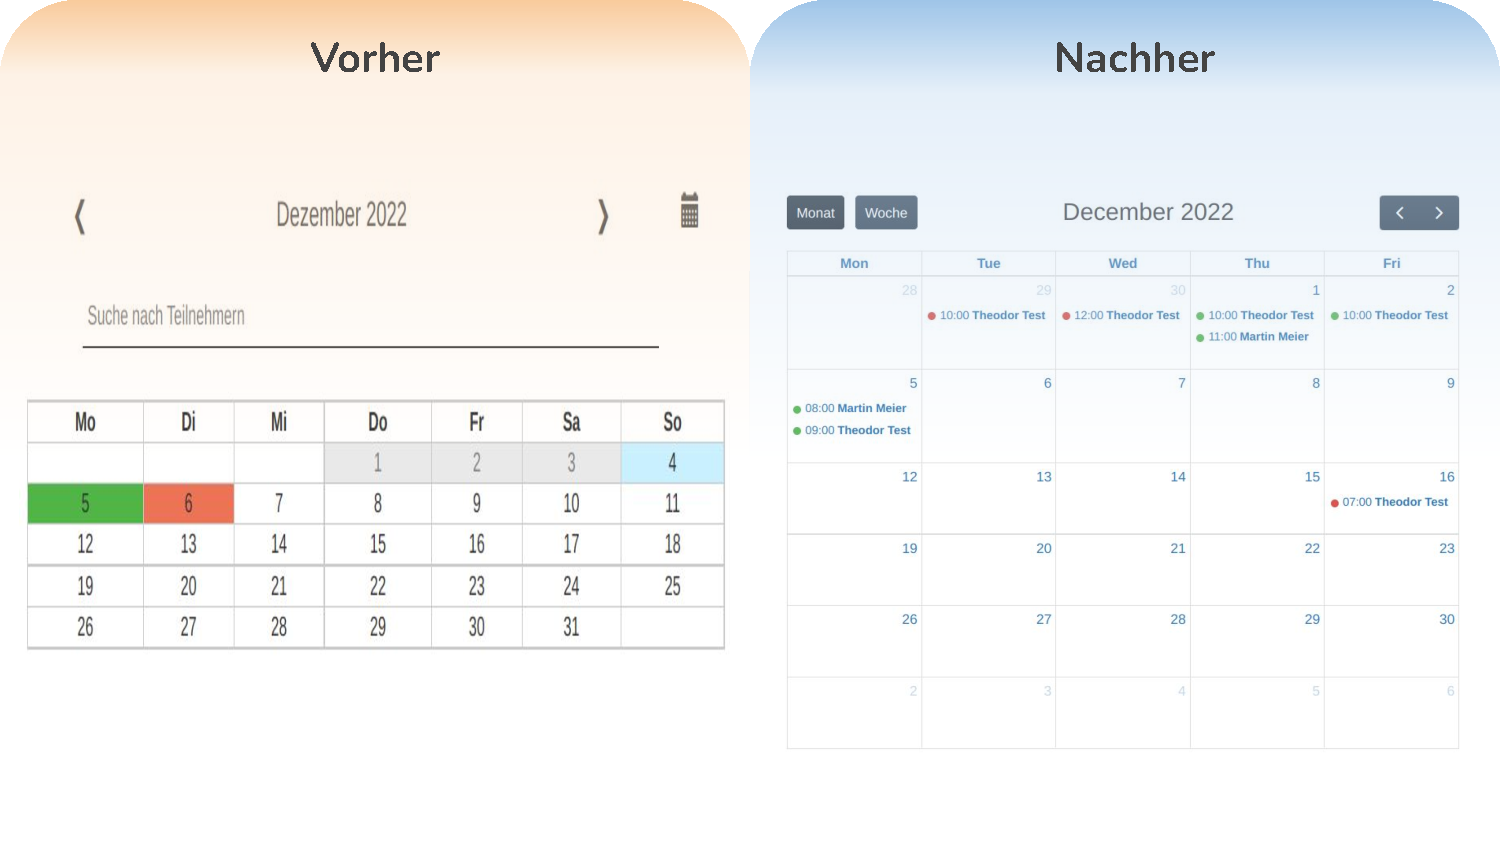
\includegraphics[width=\textwidth]{screen_past_now_month_view.pdf}
\end{figure}

Als nächstes wurde beim Interivew Im ontext deutlich, dass eine Funktion
ootwendig ist um im Nachhinein den Termin eines Ratsuchednen schnel und
unkolizert finden zu können. Hierfür wurde die Suchfunktion impementiert.
Bereist nach dem eingeben eingier Buchstaben aus dem Namen der Ratsuchednen
PErson schlägt diese neue Suchfunktion passende ERgebnisse vor und bietet in
einer tabellarischen Übersicht direkt die wichtigsten Daten zum zugehörigen
BEratungstermine. Druch einen Klick auf ein Suchergebniss kann der Termin
schnell und einfach in der Detailsansiht geöffnet werden. Im Vergleich zu alten
Softwareversion sind die Suchergebnisse sehr viel ausführlicher und
strukturierter dargestellt. Dies wurde auch im Nutzertest positiv wargenommen.
In weiteren test schein der EIndruck, dass die alte Suchfunktion etwa schneller
ergebnisse anzeigt. Dies kann aber erst objektiv bewertet werden, wenn die neue
Impemntierung auch auf den gelichen Produktiv servern installiert und im
Enisatz ist.

\begin{figure}[H]
    \caption{Vergleich der Suchfunktion in der alten und neuen Softwareversion}
    \centering
    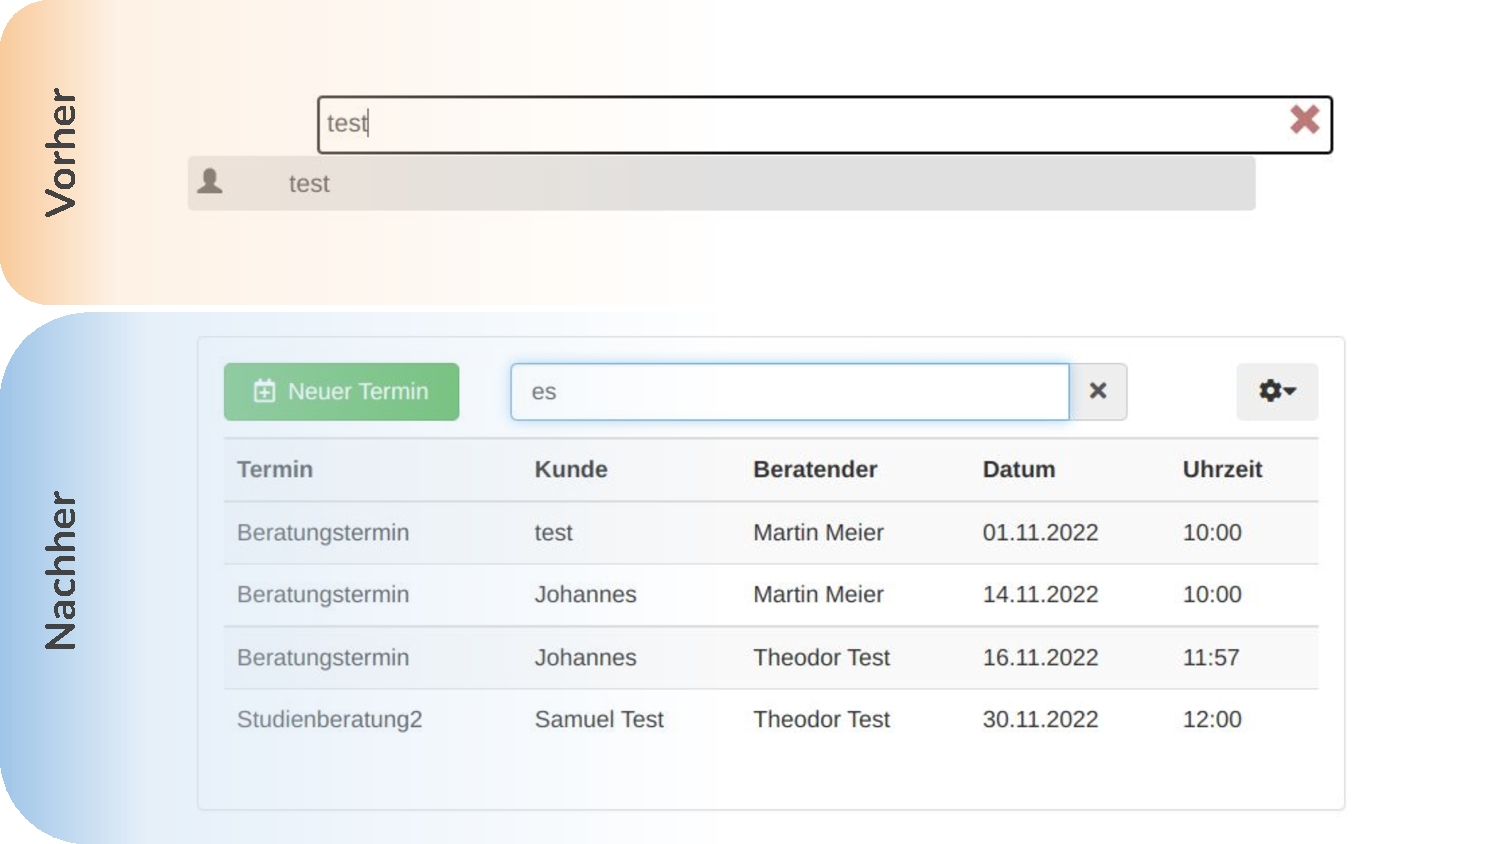
\includegraphics[width=\textwidth]{screen_past_now_search.pdf}
\end{figure}

Als letztes wurde im Anschnitt \ref{subsection:SpannendeErkenntnisse} das
elegante DArstellen der Telefonnummern gefordert. Diess Feature lieiß sich in
der PRaxis leicht impemtneiren, idem in die aus der DAtenbank abgerufenen
Telefonnummer einfach an jeder vierten Stelle ien Leerzeichen eingefügt wird.
Somit kann die telfonnummer von den Stfudienberatenden bei BEdarf in leicht zu
merkenden Viererblöcken in da sTelefno eingeben werden. Für andere
Nutzeraccounts als den zuständigen Beratenden werden persnliche Details der
Ratsuchednen nicht angezeigt. Diese Funktion gab es auch in der alten Version
ebretis, allerdings wird in der neune VEriosn statt den eigentlichen DAten ein
Hinweis angezeigt. Inde ralten Version wurde einfach agr nichts angezeigt, was
manchmal zu unsicherheiten geführt hat, b hier überhaput daten eingtragen und
jorrekt gespeichert wurden. DAs feedback aus dem Nutertest zeigt: Die neue
Vrinate braucht etwas mehr paltz auf dem Biildschirm, ist dafür aber klarer zu
verstehen und intuitiver zu erfassen. 

\begin{figure}[H]
    \caption{Vergleich der Detailansicht eines vergebenen Termins in der alten und neuen Softwareversion}
    \centering
    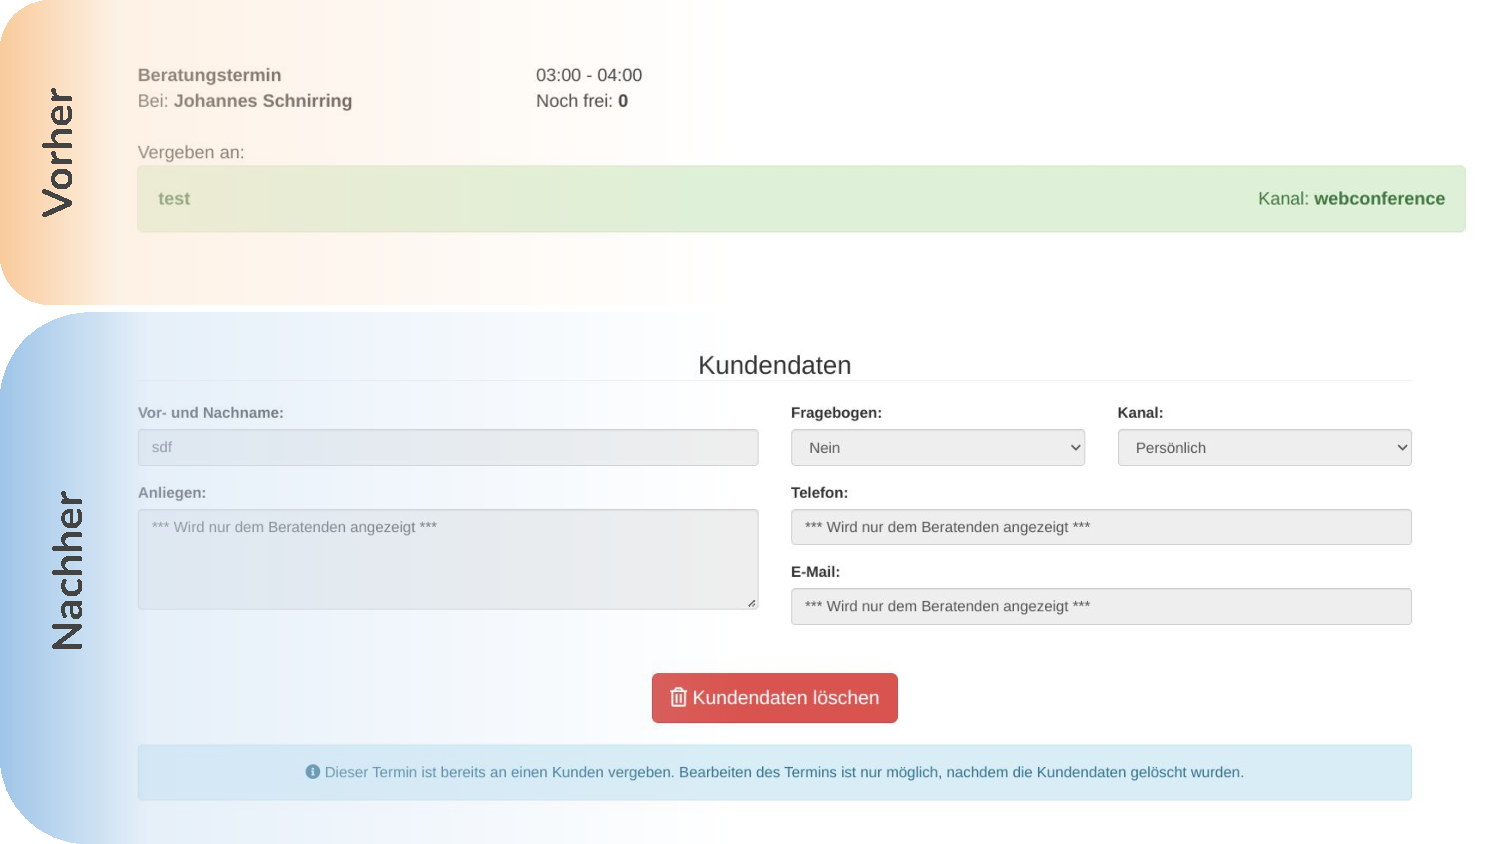
\includegraphics[width=\textwidth]{screen_past_now_client_details.pdf}
\end{figure}

\paragraph{Umsetzung von Feedback des Usertests}

\begin{figure}[H]
    \caption{Details eines vergebenen Termins aus Ansicht einer Hilfskraft.}
    \centering
    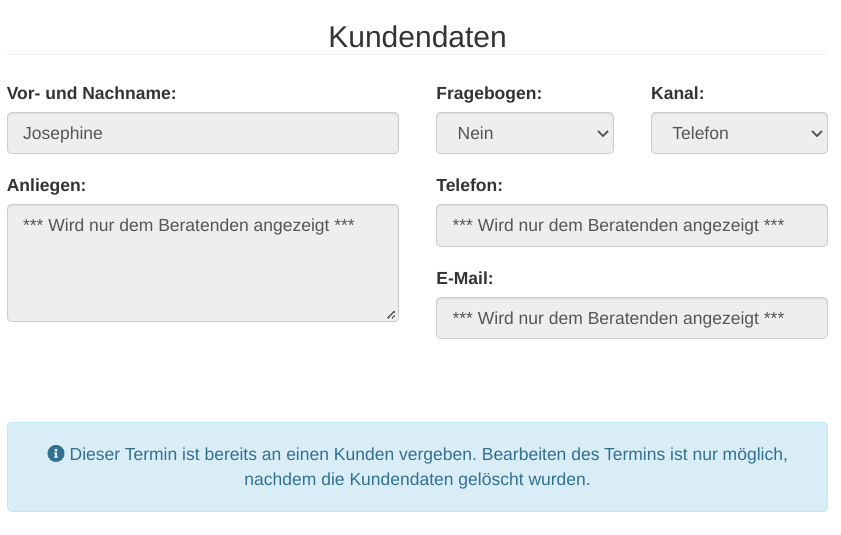
\includegraphics[width=0.9\textwidth]{screen_feedback_client_censorship.png}
\end{figure}

\begin{figure}[H]
    \caption{Neuer Button: Mit \textit{Speichern und Nächster} kann direkt der nächste Termin eingetragen werden.}
    \centering
    
\includegraphics[width=0.9\textwidth]{screen_feedback_save_next.png}
\end{figure}

\subsection{Reflektion der eingesetzen Methoden}
\label{subsection:reflection}

\paragraph{Human Centered Design und IIK}
% Einfache Umsetzung vs Nutzerfreundliche Lösung
% IIK sehr ertragreich, Prototypen wichtig für Feedback, Vorstellung

\paragraph{Implementierung und Usertests}
% Problem: Designpattern bei fertigem Softwareökosystem sehr eingeschränkt
% Fullcalendar Lib: Weniger Arbeit (billiger, robuster) dafür weniger Flexibilität
% Objektorientierter Ansatz sinnvoll für start serverlastige Anwendung?
% Evtl frühere Tests

\subsection{Zusammenfassender Abschluss}
\label{subsection:conclusion}
% Eingehen auf Fragestellung der Einleitung
% An welchen Stellen können die theoretischen Grundlagen des Human Centered Design den Entwicklungsprozess in der Praxis tatsächlich sinnvoll unterstützen? 
% Gab es eventuell auch Methoden, die in der praktischen Umsetzung problematisch waren oder noch optimiert werden könnten?
% Erfüllt die Software die gewünschten Anforderungen?
% Abrundendes Schlusswort

\subsection{Ausblick}
\label{subsection:outlook}
% Einführung neue Softwareversion (viel testen und abstimmen)
% Andere Module Überarbeiten
% Gruppentermine / Self Service einbuchen (Sicherheit)